\documentclass{article}
\usepackage{listings}
\usepackage{xcolor}
\usepackage{graphicx}

\definecolor{dkgreen}{rgb}{0,0.6,0}
\definecolor{gray}{rgb}{0.5,0.5,0.5}
\definecolor{mauve}{rgb}{0.58,0,0.82}
\definecolor{orange}{rgb}{1.0,0.5,0}

\lstset{frame=tb,
  language=Java,
  aboveskip=3mm,
  belowskip=3mm,
  showstringspaces=false,
  columns=flexible,
  basicstyle={\small\ttfamily},
  numbers=none,
  numberstyle=\color{orange},
  keywordstyle=\color{blue},
  commentstyle=\color{dkgreen},
  stringstyle=\color{mauve},
  breaklines=true,
  breakatwhitespace=true,
  tabsize=3
}

\title{Analysis of Poisson Relaxation with Threads}
\date{\today}
\author{Arthur Ceccotti - 8544173}

\begin{document}
\maketitle

\section{Introduction}
I have written a version of the \textit{Poisson's Equation} using the relaxation technique with a variable number of threads. The correctness of the program was guaranteed by checking the expected number of iterations (65,251) and also manually visualizing the array convergence over different iterations, as seen in figures \ref{fig:it0}-\ref{fig:itFinal}, produced from script XXXXX.
	
  \begin{figure}
  \centering
  \begin{minipage}{0.45\textwidth}
    \caption{0 iterations}
    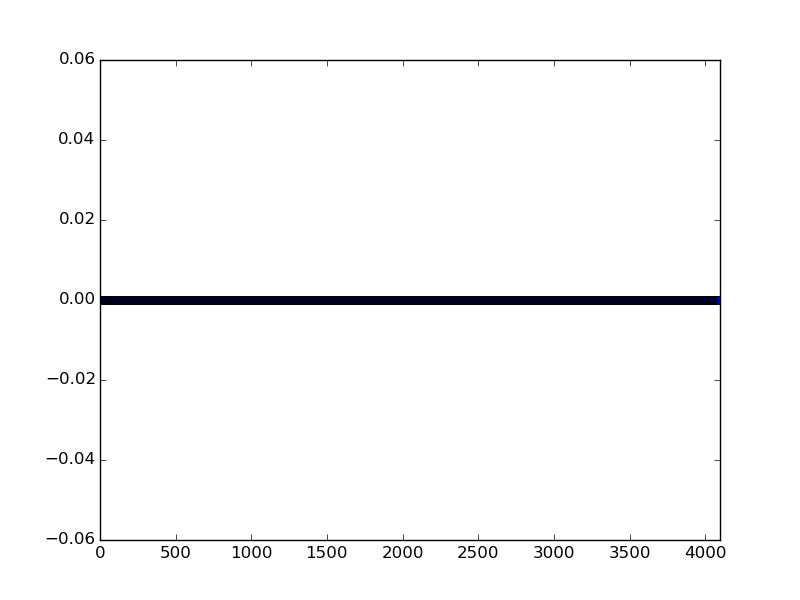
\includegraphics[width=1\linewidth, natwidth=800, natheight=600]{graphs/it1.png}
    \label{fig:it0}
  \end{minipage}
  \begin{minipage}{0.45\textwidth}
    \caption{10 iterations}
    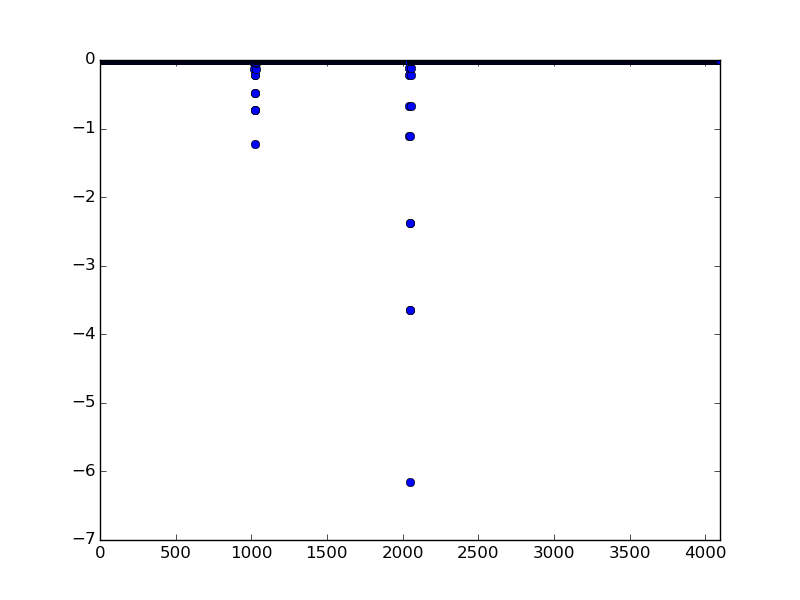
\includegraphics[width=1\linewidth, natwidth=800, natheight=600]{graphs/it10.png}
    \label{fig:it10}
  \end{minipage}
  \begin{minipage}{0.45\textwidth}
    \caption{100 iterations}
    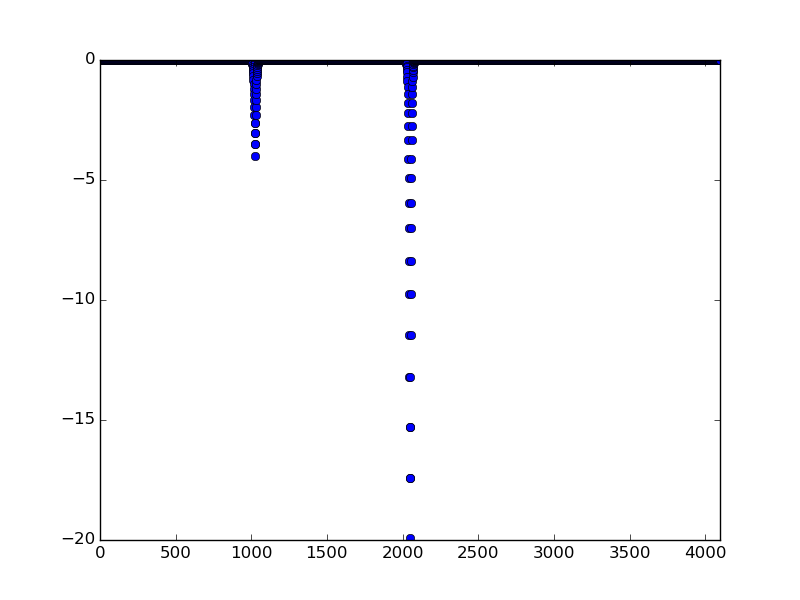
\includegraphics[width=1\linewidth, natwidth=800, natheight=600]{graphs/it100.png}
    \label{fig:it100}
  \end{minipage}
  \begin{minipage}{0.45\textwidth}
    \caption{100 iterations}
    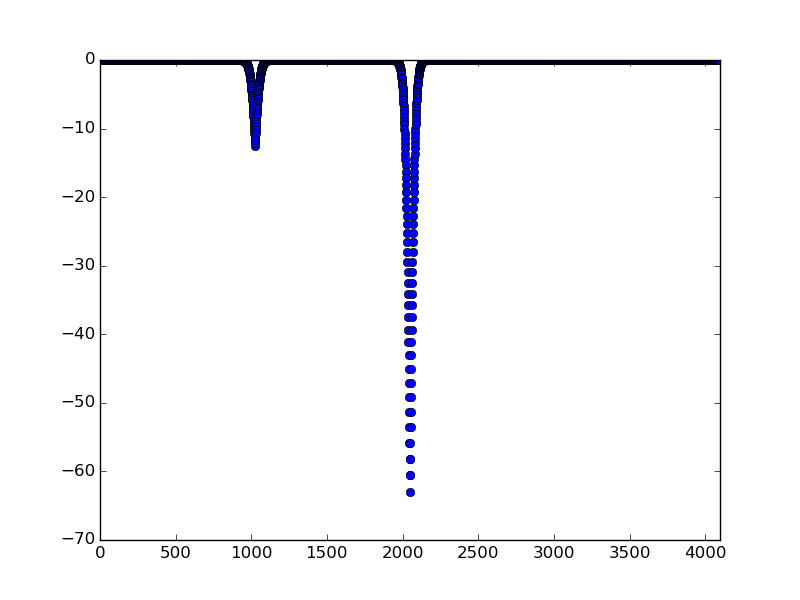
\includegraphics[width=1\linewidth, natwidth=800, natheight=600]{graphs/it1000.png}
    \label{fig:it1000}
  \end{minipage}
  \begin{minipage}{0.45\textwidth}
  \caption{10,000 iterations}
    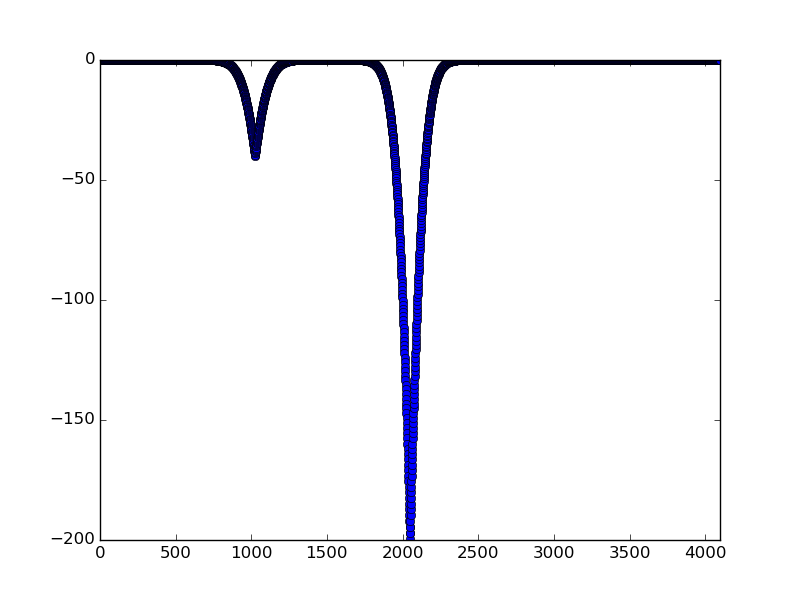
\includegraphics[width=1\linewidth, natwidth=800, natheight=600]{graphs/it10000.png}
    \label{fig:it10000}
  \end{minipage}
  \begin{minipage}{0.45\textwidth}
    \caption{65,250 iterations}
    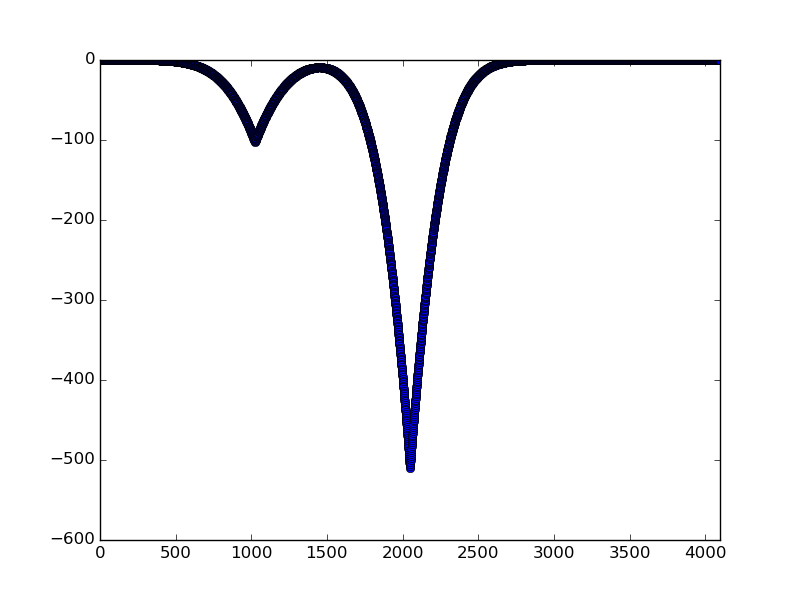
\includegraphics[width=1\linewidth, natwidth=800, natheight=600]{graphs/itFinal.png}
    \label{fig:itFinal}
  \end{minipage}
  \end{figure}	

Intermittent performance drops/spikes were reduced by running every instance 10 times, allowing the gathering of average values and standard deviation. The large amount of data produced from all the runs was analysed and plotted by my Python script under listing \ref{lst:pythonscripts}. The data plots were a consequence of running the given program on \textit{mcore48.cs.man.ac.uk}. \footnote{\label{machinespecs} \\
  Dell/AMD quad 12-core (48 cores total), each with specs:\\
  model name: AMD Opteron(tm) Processor 6174 \\
  clock speed: 2.2 GHZ \\
  cache size: 512 KB \\}

\section{Evaluation}

\iffalse


  Upon writting a version of the Poisson's Equation Approximation program with threads
  
  On an instance of this problem, one would expect linear speed up of performance with the increase of threads, as load is equal for every thread and there are enough hardware processors. This means, with the same vector size, 10 threads should run twice faster than 5 threads. This O(\textit{n}) speedup is certainly not true for the sorting of small vectors, because of overheads such as \textbf{thread initialisation time} (which includes OS calls, stack memory assignment for the thread, adding it to the JVM data structure,...) and \textbf{joins}. This meas the overall thread creation bottleneck may take longer than the sorting itself. This is a very similar behaviour to the previous coursework for Vector Addition with Threads.

  For small vector sizes, the increase of number of threads to solve the problem in fact decreases performance, as can be seen on figures \ref{fig:1000} and \ref{fig:10000} for vector sizes of \textit{1000} and \textit{10,000}. In these cases the program has its best performance with a single thread sorting the whole array sequentially, which saves having to spawn threads which will take milliseconds to initialise and quickly die after doing very few operations.

  \begin{figure}
  \centering
  \begin{minipage}{0.45\textwidth}
    \caption{1,000 elements}
    \includegraphics[width=1\linewidth, natwidth=800, natheight=600]{evaluation/graphs/1000.png}
    \label{fig:1000}
  \end{minipage}
  \begin{minipage}{0.45\textwidth}
    \caption{10,000 elements}
    \includegraphics[width=1\linewidth, natwidth=800, natheight=600]{evaluation/graphs/10000.png}
    \label{fig:10000}
  \end{minipage}
  \end{figure}

  The balance of thread overhead and speedup is reached at \textit{100,000}-\textit{1,000,000} vector sizes, as seen on figures
  \ref{fig:100000} and \ref{fig:1000000} respectively, where adding more threads does not significantly increase performance, as it introduces similar slowdown. Because of this the graphs present wide error bars and an overall horizontal performance. 

  \begin{figure}
  \centering
  \begin{minipage}{0.45\textwidth}
    \caption{100,000 elements}
    \includegraphics[width=1\linewidth, natwidth=800, natheight=600]{evaluation/graphs/100000.png}
    \label{fig:100000}
  \end{minipage}
  \begin{minipage}{0.45\textwidth}
    \caption{1,000,000 elements}
    \includegraphics[width=1\linewidth, natwidth=800, natheight=600]{evaluation/graphs/1000000.png}
    \label{fig:1000000}
  \end{minipage}
  \end{figure}

  The advantage of threads can be finally seen on large instances of the problem with \textgreater\textit{10,000,000} elements, as described on figures \ref{fig:10000000} and \ref{fig:100000000}. Joins and initialisation still pose as an overheads, but are insignificant given the amount of sorting performed.

  \clearpage

  \begin{figure}
  \centering
  \begin{minipage}{0.45\textwidth}
    \caption{10,000,000 elements}
    \includegraphics[width=1\linewidth, natwidth=800, natheight=600]{evaluation/graphs/10000000.png}
    \label{fig:10000000}
  \end{minipage}
  \begin{minipage}{0.45\textwidth}
    \caption{100,000,000 elements}
    \includegraphics[width=1\linewidth, natwidth=800, natheight=600]{evaluation/graphs/100000000.png}
    \label{fig:100000000}
  \end{minipage}
  \end{figure}

  \section{Code}
    \subsection{Java Unit Tests}
      \lstinputlisting[language=Java,
                       caption=MergeSort Unit Tests,
                       label={lst:mergesortunit}]{src/MergeSortTest.java}

    \subsection{Java Merge Sort Program}
      \lstinputlisting[language=Java,
                       caption=MergeSort Main class,
                       label={lst:mergesort}]{src/MergeSort.java}

      \lstinputlisting[language=Java,
                       caption=MergeSort Thread class,
                       label={lst:mergesortthread}]{src/MergeSortThread.java}

    \subsection{Data Evaluation Scripts}  
      \lstinputlisting[language=bash,
                       caption=Bash scripts to run MergeSort with multiple parameters,
                       label={lst:bashscripts}]{src/DemoTuca.sct}
      \lstinputlisting[language=Python,
                       caption=Python scripts to gather and plot results,
                       label={lst:pythonscripts}]{src/process.py}
                       
\fi
\end{document}